%!TEX root = ../main.tex

\section{Choices and Comparisons}\label{section:comparisons}

We here give a rationale for design decisions and the chosen system model, as well as an explanation of known advantages and limitations compared to other options and approaches.
$\frost$ is backwards compatible with any protocol using the FIPS186-5 verifier. 
This is the NIST standardised Edwards-curve Digital Signature Algorithm (EdDSA) digital signature scheme \cite{EdDSA}.
EdDSA is a variant of Schnorr signature based on twisted Edwards curves.
No changes to existing implementations of the signature format or the verifier are required.
The signing procedure, however, is changed to support threshold signers.

In \cref{table:comparisons} we compare $\frost$ with other approaches in the literature.
We limit our comparisons to other concurrently secure threshold signatures that are also backwards compatible with FIPS186-5.
This includes
\begin{itemize}
	\item An unnamed protocol by Gennaro, Jarecki, Krawczyk and Rabin \cite{GennaroJKR01}
	\item An unnamed protocol by Stinson and Strobl \cite{StinsonS01}
	\item $\mathsf{2SCHNORR}$ by Nicolosi, Krohn, Dodis, and Mazi\`eres \cite{NicolosiKDM03}
	\item $\mathsf{CLASSICS}$ and $\mathsf{ZEROS}$ by Makriyannis \cite{Makriyannis22}	
	\item An unnamed protocol by Lindell \cite{Lindell22}
	\item $\mathsf{ROAST}$ by Ruffing, Ronge, Jin, Schneider{-}Bensch, and Schr{\"{o}}der \cite{RuffingRJSS22}
	\item $\mathsf{SPARKLE}$ by Crites, Komlo, and Maller \cite{CritesKM23}
	\item $\mathsf{SPRINT}$ by Benhamouda, Halevi, Krawczyk, Rabin and Ma \cite{BenhamoudaHKRM23}
	\item $\mathsf{ARTIC}$ by Komlo and Goldberg \cite{KomloG24}
	\item $\mathsf{HARTS}$ by Bacho, Loss, Stern and Wagner \cite{BachoLSW24}
\end{itemize}

There exist some multi-signature schemes in which the signature format is compatible with FIPs186-5 but the signature verifier is incompatible.
This includes
\begin{itemize}
	\item $\mathsf{MSDL}$ by Boneh, Drijvers, and Neven  \cite{BonehDN18}
	\item $\mathsf{MuSig}$ by Maxwell, Poelstra, Seurin, and Wuille \cite{MaxwellPSW19}
	\item $\mathsf{MuSig2}$ by Nick, Ruffing, and Seurin \cite{NickRS21}
	\item $\mathsf{MuSigDN}$ by Nick, Ruffling, Seurin, and Wuille \cite{NickRSW20}
\end{itemize}
We also exclude these schemes from our comparisons in this section.

\subsection{Key for \cref{table:comparisons}}\label{section:comparisons:tablekey}
We here give a key for understanding the comparisons in \cref{table:comparisons}.
Where applicable we follow the keys in the Call for Proposals.
\begin{itemize}
	\item The number of parties $n$ can either be:
	\begin{itemize}
		\item (2) ``two" for $n = 2$;
		\item (3) ``three" for $n = 3$;
		\item  (S) ``small" for $4 \leq n \leq 8$;
		\item  (M) ``medium" for $9 \leq n \leq 64$;
		\item (L) ``large" for $65 \leq n \leq 1024$; 
		\item (E) ``enormous" for $n > 1024$.
	\end{itemize}
	\item The corruption proportion $f/n$ can either be:  
		\begin{itemize}
			\item  (D) ``dishonest majority" for $f \geq n/2$; 
			\item  (h) ``honest majority” for $f < n/2$; 
			\item (H) “two-thirds honest majority” for $f < n/3$.
	\end{itemize}
	\item The assumptions can  be:
		\begin{itemize}
			\item $\dl$ ``discrete logarithm" if the $\dl$ assumption is required;
			\item $\aomdl$ ``Algebraic one more discrete logarithm" if the $\aomdl$ assumption is required.
		\end{itemize}
	\item 	The idealisation for all schemes includes the random oracle model and so this is not indicated in the table.  The additional idealisations can be:
		\begin{itemize}
			\item (G)  ``game based" for a game based security notion;
			\item (S) ``simulation" for a simulation based security notion;
			\item (AGM) ``algebraic group model" if the AGM is required.
		\end{itemize} 
 	\item The liveness guarantees can be
 		\begin{itemize}
 			\item  (IA) ``identifiable abort" if cheating parties can be identified;
 			\item  (h) ``robust under honest majority” if robustness holds given $f < n/2$;
 			\item (N) ``not robust against active adversaries". 
 		\end{itemize}
 	\item The adversary for all schemes we consider is active.  We write:
 		\begin{itemize}
 			\item (U)  ``unknown" for no known positive or negative adaptive result; 
 			\item (H) ``half" if adaptive security is provable for $f \leq \frac{k}{2}$
 			\item (F) ``full" for full adaptivity security i.e. adaptive security if provable for $f = k - 1$.
 		\end{itemize}
 	\item The number of rounds  can either be:
 	\begin{itemize}
 		\item (2) ``two" for $2$ rounds;
 		\item (3) ``three" for $3$ rounds;
 	\end{itemize}
 	\item The distributed system and communication requirements can be ......
 	\item The key generation can be ......
\end{itemize}   

\subsection{Concurrency}\label{section:comparisons:concurrency}
$\frost$ as well as all other schemes in this comparison is concurrently secure.  
There are no restrictions on the number of sessions a polynomial time adversary can have open at the same time.
This is a strict requirement in the call for proposals.

\subsection{Threshold Profiles}
$\frost$ is a $k$-out-of-$n$ threshold signature that supports any $1 \leq k \leq n$.
As in the Call for Proposals \cite{} we have: $k$ is the number of participants requires to sign; $f$ is the corruption proportion; and  $n$ is the number of parties.
The number of parties is enormous ($n > 1024$) although smaller $n$ is also supported.
The corruption proportion is dishonest majority ($f \geq \frac{n}{2}$) although smaller $f$ is also supported.
$\frost$'s corruption threshold is equal to the participation-minus-1 threshold $f = k-1$.
\mary{This may not be true for potential adaptive security reduction.}


\subsection{Security Assumptions}\label{section:comparisons:security}
$\frost$ is secure under the Algebraic-One-More-Discrete-Logarithm ($\aomdl$) problem \cite{NickRS21}.
This is a falsifiable assumption that holds in the generic group model \cite{CorettiDG18,BauerFP21}.
It is strictly better than the non-falsifiable One-More-Discrete-Logarithm problem \cite{BellareNPS03} because the adversary can only query on known linear combinations of fixed challenges,
as opposed to any group element.
It is strictly worse than the discrete-logarithm $(\dl)$ assumption under which the base EdDSA signature is secure.
An adversary that solves $\dl$ can also solve $\aomdl$, but an adversary that solves $\aomdl$ cannot necessarily solve $\dl$.

$\frost$ generates EdDSA signatures which cannot be post-quantum secure, because EdDSA depends on the discrete logarithm assumption.
There is a known quantum attack against the discrete logarithm problem \cite{Shor99}.



\subsection{Security Idealisation}\label{section:comparisons:idealisation}
The security reduction for $\frost$ is given under a game-based security formulation in the programmable random oracle model.
It is expected the idealised model for any threshold protocol producing EdDSA signatures must be stronger than the standard model.
This is because there is no security reduction for EdDSA without any random oracle~\cite{PaillierV05,FischlinF13,FleischhackerJS14}

There is no known security reduction for $\frost$ in the universal composability model.
To minimise the risks of composability attacks when $\frost$ is used in larger protocols,
it is important to prefix the hash digests with appropriate domain separators.
We fully specify the recommended domain separators in this document.

\subsection{Liveness}
$\frost$ is not  robust because there are no guarantees that any given session will terminate.
If a session does not terminate then this does not effect the unforgeability security guarantees.
$\frost$ does satisfy identifiable abort.  This means that if any party does not follow the honest signing protocol then they can be actively detected and removed from future iterations of the protocol.

\mary{Say something about robust competitors.}

\subsection{Adversary}\label{section:comparisons:adversary}
$\frost$ is actively secure.  An adversary can corrupt up to $f$ parties, controlling them to arbitrarily deviate from the prescribed multi-party protocol.
There is no adaptive security reduction for $\frost$, i.e., we cannot prove security against an adversary that can decide which parties to corrupt after observing some of the protocol execution.
However there is also no known adaptive attack against $\frost$.

\mary{
	Please help, I know little about this:
	The proposed threshold schemes should be compatible with modular subprotocols / mechanisms for proactive (and reactive) recovery, which attempt to recover possibly corrupted parties back to an uncorrupted state. This is especially important to better handle a persistent mobile adversary that continuously attempts to corrupt more parties. With respect to refreshing secret shares, the solutions can be based on a modularized phase of secret-resharing (see T6), while also specifying the needed conditions (e.g., requirement of some initial/final agreement by a qualified quorum) for its integration.
}

There exist $3$ round schemes that provably fully adaptive \cite{} in the algebraic group model with non-programmable random oracles.  However there is no static or adaptive security reduction of $\frost$ in this model.  

\subsection{Number of Rounds}\label{section:comparisons:rounds}
$\frost$ has $2$ signing rounds and allows the message to be determined in the second round of signing.
Thus $\frost$ allows for an effective non-interactive signing procedure assuming that a preprocessing phase is run in advance.
This is not possible for any threshold scheme producing EdDSA signatures that depends on $\dl$.

Currently there is no known efficient concurrently secure $2$-round threshold signature scheme that generates EdDSA signatures that is secure under $\dl$.
We do not know if this is fundamental or not.  However, there are efficient concurrently secure $3$-round threshold signature schemes \cite{Lindell22,Makriyannis22,CritesKM23}.
The $3$ round schemes require the message to be fixed in the first or second round of the protocol.

\subsection{Communication Complexity}\label{section:comparisons:communicationcomplexity}
A full theoretical and experimental break down of the communication complexity of $\frost$ is given in \cref{?}.
In each signing session all parties:  send $2 \Gr$ and $1 \F$; and receive $2 k \Gr$ as well as the message and signing set.

\subsection{State Management and Storage Requirements}\label{section:comparisons:statemanagement}
$\frost$ requires state management to ensure that:
(1) secret randomness from the first round is available to the signer in the second round;
(2) nonces from the first round are not used twice.
All schemes we compare against also require state management to ensure these two properties.
If the secret randomness from the first round is lost then the signer will not be able to take part in the second round.
If the nonces from the first round are used twice then an adversary can recover the signers partial secret key,
thus compromising the signer.

Unlike in FIPS186-5 it is important that nonces are not generated using deterministic randomness to prevent nonces from the first round being used twice.

As a two round scheme $\frost$ has simpler state management than the other threshold signatures we compare against.
For example $\frost$ does not need to track which round of signing each party is currently in.
There are no single round threshold signatures that product FIPS186-5 signatures.

To allow simulate non-interactive signing $\frost$ preprocesses numerous first round contributions for each signing party.
This is possible because $\frost$ signers do not learn the message or signing set until the second round.
This requires storage of the state for all (preprocessed) open sessions.
We only analyse security when the states are stored and managed exactly as specified in this document.
\mary{Check with others if this is okay.}
\liz{Is state updated, or is state maintained for each round?}

\subsection{Distributed Systems and Communication}



\subsection{Key Generation}\label{section:comparisons:keygeneration}
For simplicity we specify $\frost$ assuming a trusted setup procedure, where a single trusted user generates all key shares.
For many applications such as backups this suffices.
However  $\frost$ can be instantiated with any simulatable distributed key generation \cite{}.

\begin{table}[htbp]
	\centering
	\begin{tabular}{c c c c c c c c}
		\toprule
		Scheme & \ $n$ \ & $f/n$ & Assumption & Ideal & Live & Adversary & Rounds \\ \midrule
		GJKR01 \cite{GennaroJKR01}& & & & & & & \\ 
		SS01 \cite{StinsonS01} & & & & &  & & \\
		$\mathsf{2SCHNORR}$ & & & & & &  & \\
		$\mathsf{CLASSICS}$ & & & & & & & \\
		$\mathsf{ZEROS}$ & & & & & &   & \\
		Lindell22 \cite{Lindell22} & E & D & $\dl$ & S &  IA, N & U & $3$ \\
		$\mathsf{ROAST}$ & & & & &  & & \\
		$\mathsf{SPARKLE}$ & E & D & $\dl$ & G & IA, N & H & $3$ \\
		$\mathsf{SPARKLE}^*$ & E & D & $\dl$ & G, AGM & IA, N & F & $3$ \\
		$\mathsf{SPRINT}$ & & & & & &  & \\
		$\mathsf{ARTIC}$ & & & & & &  & \\
		$\mathsf{HARTS}$ & & & & & &  & \\
		\midrule 
		$\mathsf{FROST}$ & E & D & $\aomdl$ & ROM & IA, N & U & $2$ \\
		\bottomrule
	\end{tabular}
	\caption{\label{table:comparisons}
		Table of comparisons with other schemes that are backwards compatible with the signature format and verifier of FIPS186-5.
		We provide a key for interpreting this table in \cref{section:comparisons:tablekey}.
	 }
\end{table}


\section{System Model}\label{section:system-model}

\subsection{Participants}
We consider a set of $n$ parties
$P_1, \dots, P_n$ and a coordinator $\mathcal{C}$, which execute the FROST signing protocol.
The coordinator may be one of the parties $P_i$ or an external party.
All parties can be modeled as probabilistic, polynomial-time Turing machines.
We assume there is prior agreement on the value of $n$ and the threshold $t$ as well as the $n$ participant identifiers (i.e., all parties ``know who" the $n$ parties are).
In implementations with authenticated channels, participant identifiers may be associated to public keys, which need to be verified, for example, by zero-knowledge proofs during key generation.

Note that FROST can be instantiated without the coordinator $\mathcal{C}$ by having parties broadcast their protocol messages instead.  However, this would result in increased communication complexity of $\BigO(\kappa n^2)$, where $\kappa$ is the security parameter.

\subsection{Distributed Systems and Communication}

\begin{description}

\item[Synchrony.] FROST is unforgeable even in an asynchronous network. An adversary may be \emph{rushing}; that is, it may wait until all honest protocol messages have been sent before determining its own messages.

\item[Reliability.] FROST relies on a reliable network channel, meaning that all protocol messages are delivered correctly, exactly once, and in the intended order.  \liz{The NIST document says we should discuss the pitfalls of deployment in environments with weaker guarantees (e.g., with asynchronous and unreliable channels), and possible mitigations.  What are some possible mitigations against forging if the network is unreliable?}

\item[Broadcast.] FROST does not rely on a broadcast channel; an adversary may send inconsistent protocol messages to honest parties, even within the same signing session.  Furthermore, authenticated channels are not assumed either; an adversary, who may control the coordinator $\C$, can decide which protocol messages to send to an honest party on behalf of another honest party.

\end{description}

\noindent \textbf{Robustness.} FROST is not robust, meaning that there is no guarantee that a signing session will terminate.
However, in a slightly stronger network model, FROST does achieve identifiable aborts.
Indeed, if authenticated channels are assumed, participant identifiers may be associated to public keys via a public key infrastructure (PKI).
Then, if a signer produces a malformed protocol message, they may be identified and removed from the signing session, and a new FROST session may be initiated without them.
While this yields a robust protocol overall, these sequential iterations of FROST additionally require the network to be synchronous.

\subsection{Adversary}

A threshold signature scheme is said to be \emph{secure} if, with overwhelming probability, an adversary cannot forge a threshold signature.

\begin{description}

\item[Active.] FROST is secure against an active adversary who may corrupt up to $f = t-1$ out of a threshold of $t$ parties (where $t \leq n$), controlling them to arbitrarily deviate from the prescribed multi-party protocol.   As described in Section~\ref{sec:unforgeability}, FROST achieves TS-(S)UF-3 security~\cite{BellareCKMTZ22} (without authenticated channels).

\item[Adaptive.] The stronger adaptive adversary is able to decide which parties to corrupt after observing some of the protocol execution. 
Upon corruption, the adversary learns the secret key and private state for the corrupted party in all open signing sessions.
Currently, there is no known proof of adaptive security for FROST.

\item[Mobile.] A mobile adversary ``persistently continues (attempting to) corrupt parties across multiple executions of the main protocol, possibly corrupting parties after they have been recovered from a previous corruption."
Currently, there is no known security proof for FROST capturing a mobile adversary.
\liz{Dynamic-FROST (https://eprint.iacr.org/2024/896) possibly achieves this.}

\end{description}

\subsection{HARTS}

\begin{figure}
    \centering
    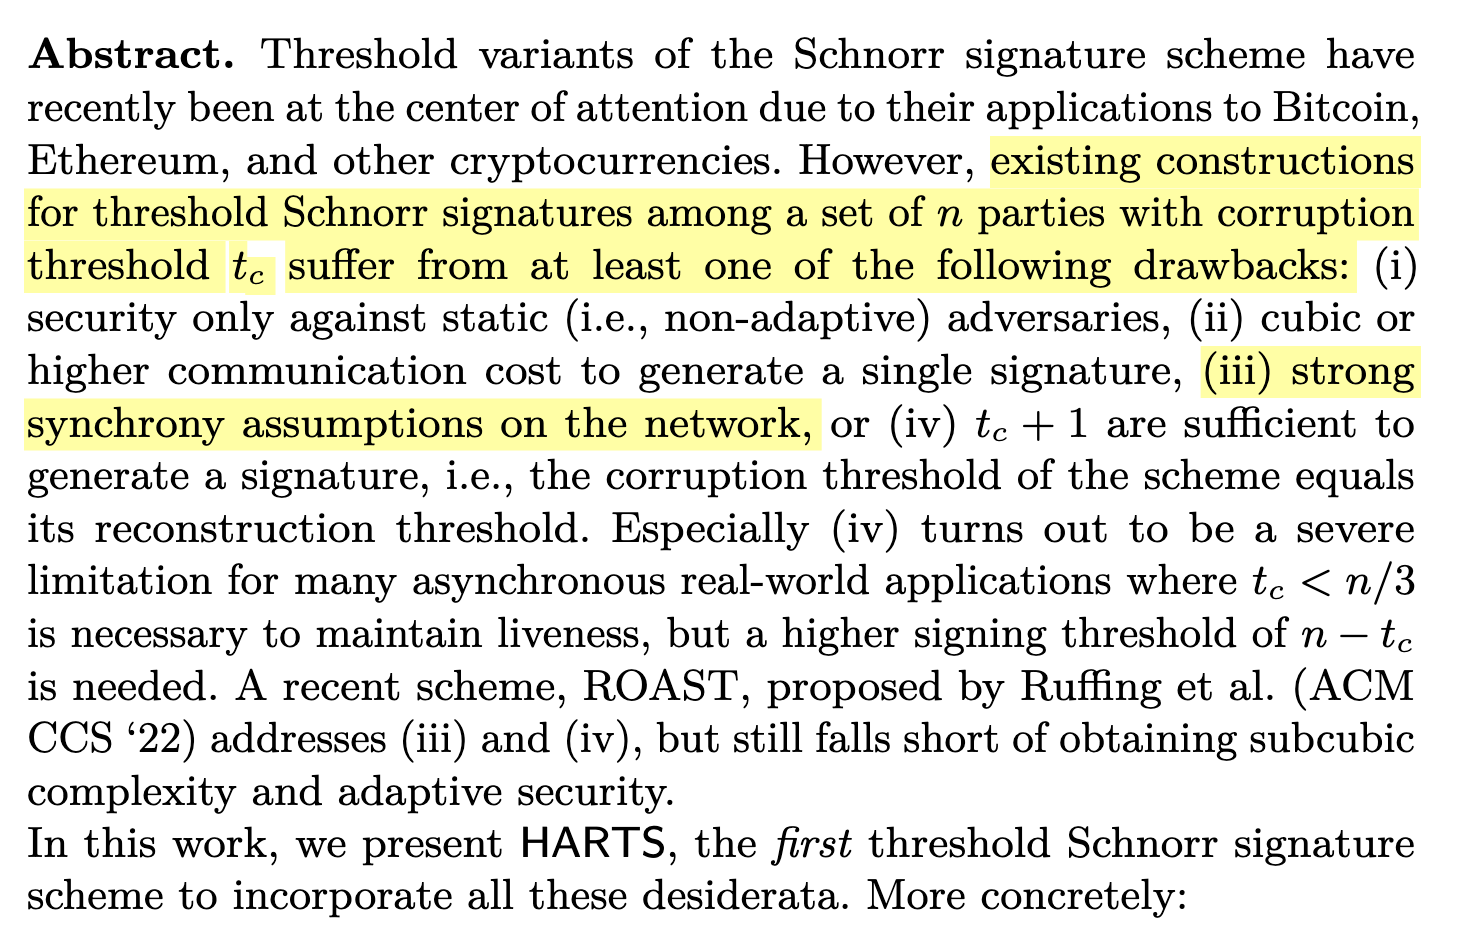
\includegraphics[width=1\linewidth]{images/HARTS_abstract.png}
    \caption{HARTS abstract claiming ``strong synchrony assumptions" in other works.}
\end{figure}

\begin{figure}
    \centering
    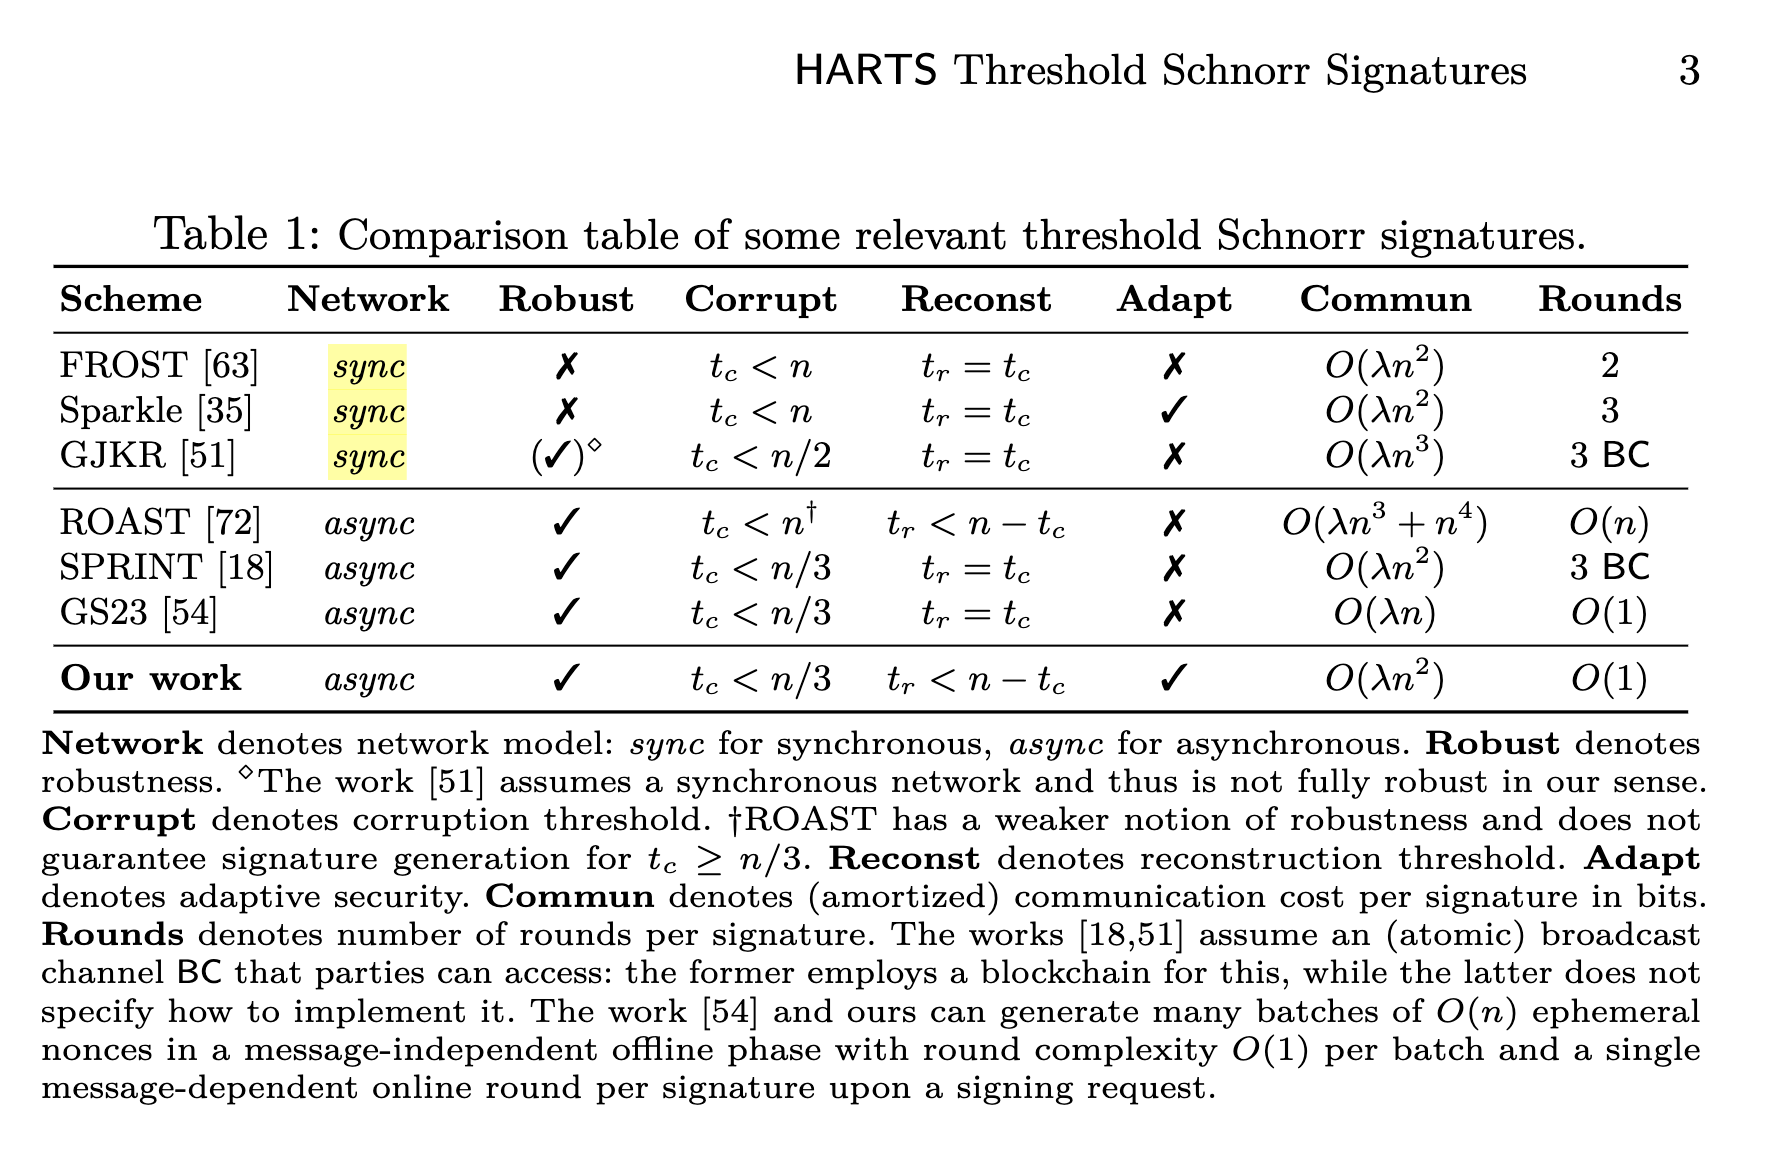
\includegraphics[width=1\linewidth]{images/HARTS_table.png}
    \caption{FROST and Sparkle are \textbf{not} forgeable in an asynchronous network, whereas GJKR is \textbf{forgeable}.}
\end{figure}

\begin{figure}
    \centering
    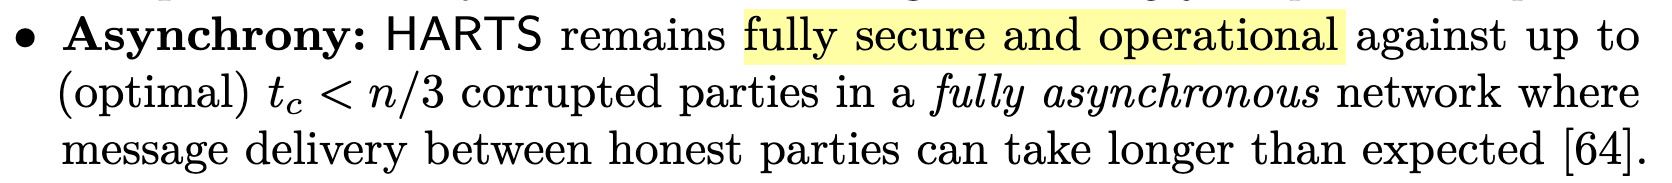
\includegraphics[width=1\linewidth]{images/HARTS_async_defn.png}
    \caption{HARTS definition of asynchrony. It is not clear what ``fully secure and operational" means.}
\end{figure}

\begin{figure}
    \centering
    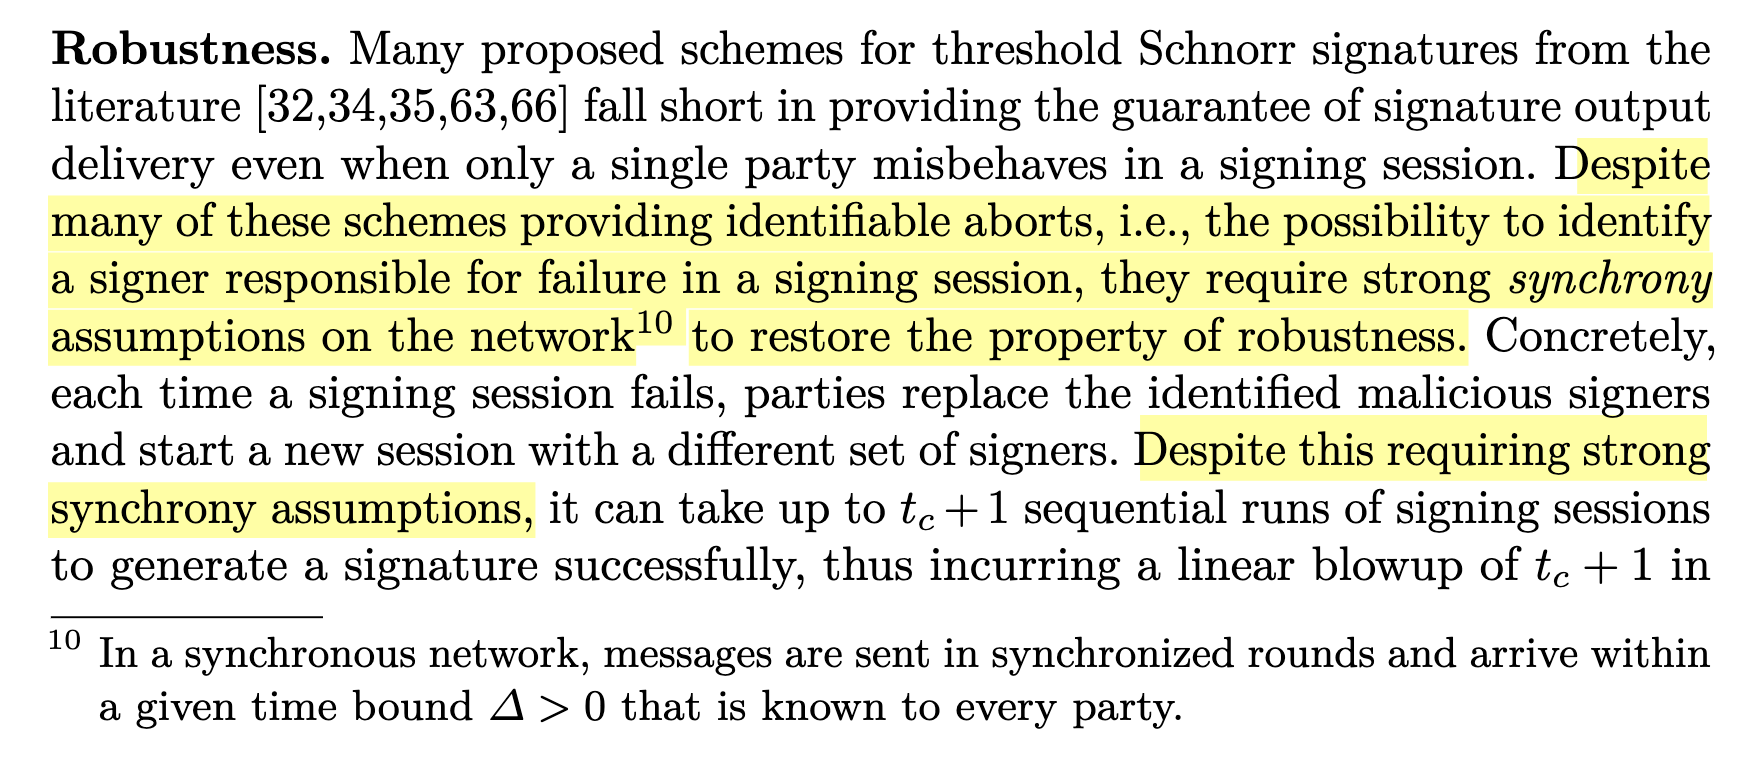
\includegraphics[width=1\linewidth]{images/HARTS_appendix.png}
    \caption{A more accurate description, buried in the appendix of HARTS, which says that synchrony is needed to restore robustness.  However, it appears to claim synchrony is needed even for just identifiable aborts.}
\end{figure}

\newpage

\subsection{SPRINT: https://eprint.iacr.org/2023/427}

\begin{figure}
    \centering
    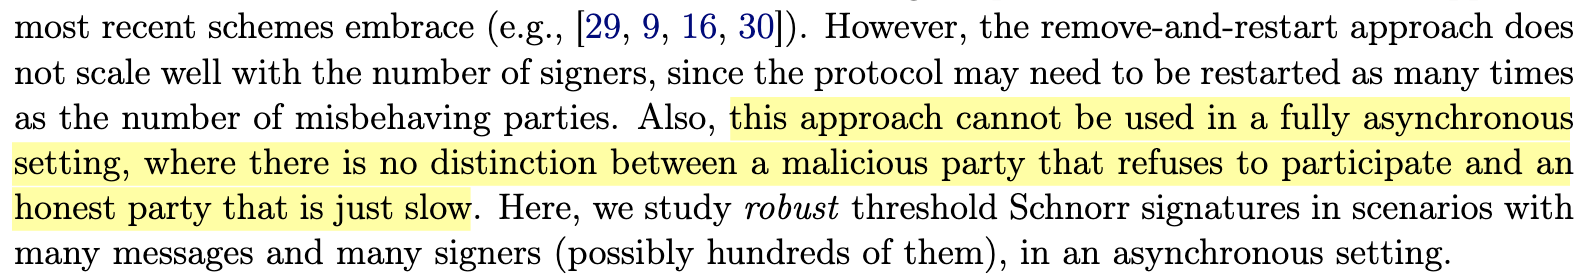
\includegraphics[width=1\linewidth]{images/SPRINT_IA.png}
    \caption{SPRINT, like HARTS, identifies synchrony as being needed for identifiable aborts.}
\end{figure}

\begin{figure}
    \centering
    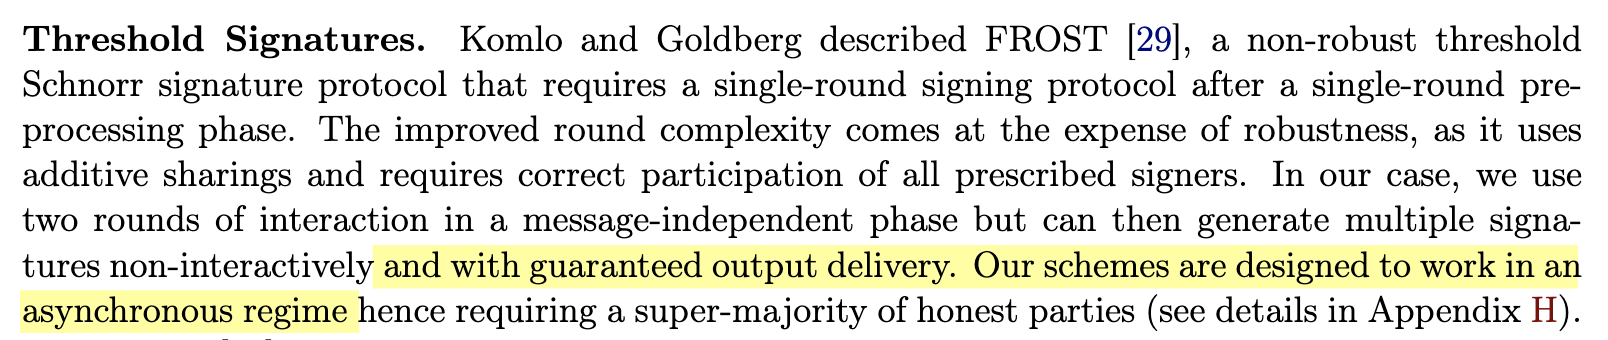
\includegraphics[width=1\linewidth]{images/SPRINT_FROST.png}
    \caption{SPRINT is a bit unclear about asynchrony.}
\end{figure}

\newpage

\subsection{ROAST: https://eprint.iacr.org/2022/550}

\begin{figure}
    \centering
    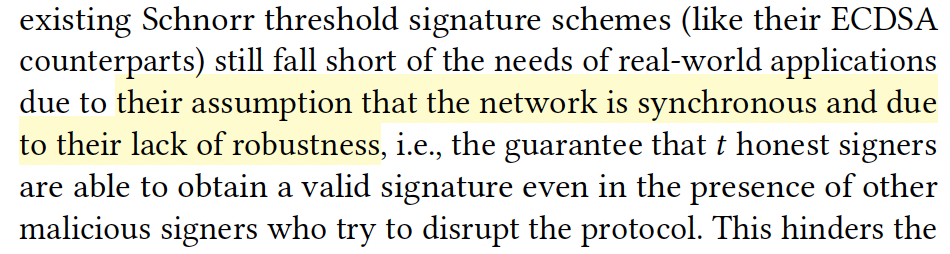
\includegraphics[width=1\linewidth]{images/ROAST_abstract.png}
    \caption{ROAST abstract says prior schemes assume synchrony.}
\end{figure}

\begin{figure}
    \centering
    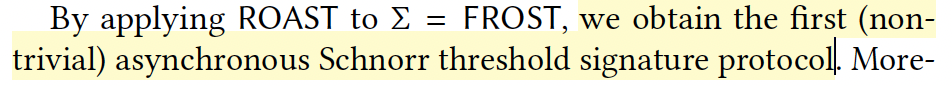
\includegraphics[width=1\linewidth]{images/ROAST_first_async.png}
    \caption{ROAST claiming to be first asynchronous threshold Schnorr scheme.}
\end{figure}

\begin{figure}
    \centering
    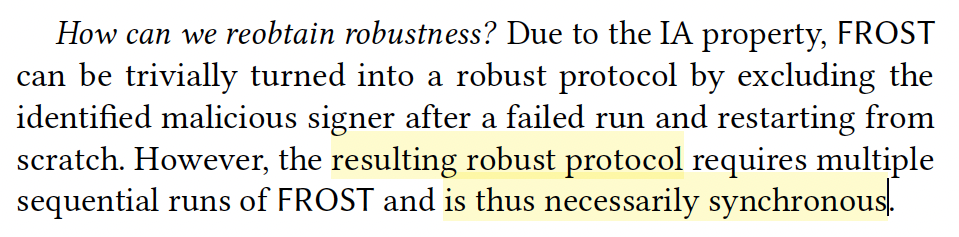
\includegraphics[width=1\linewidth]{images/ROAST_IA.png}
    \caption{Synchrony is required for the IA property of FROST.}
\end{figure}

\begin{figure}
    \centering
    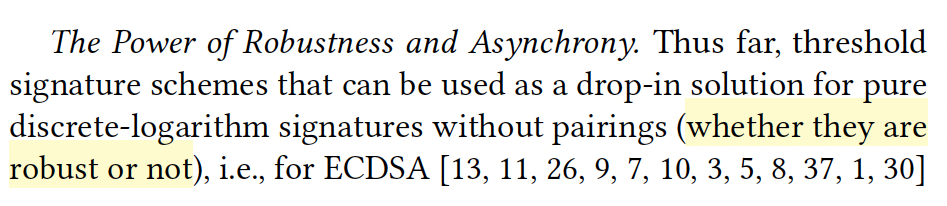
\includegraphics[width=1\linewidth]{images/ROAST_sync_reqd.png}
    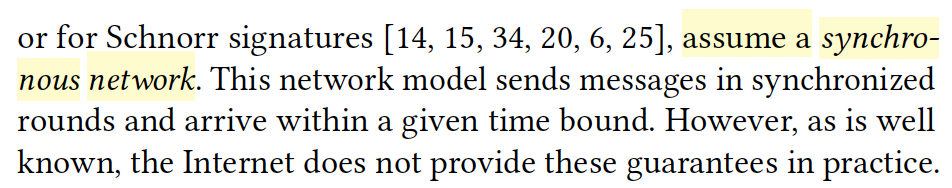
\includegraphics[width=1\linewidth]{images/ROAST_sync_reqd2.png}
    \caption{ROAST claims prior works required synchrony \textbf{whether they are robust or not}.}
\end{figure}

\begin{figure}
    \centering
    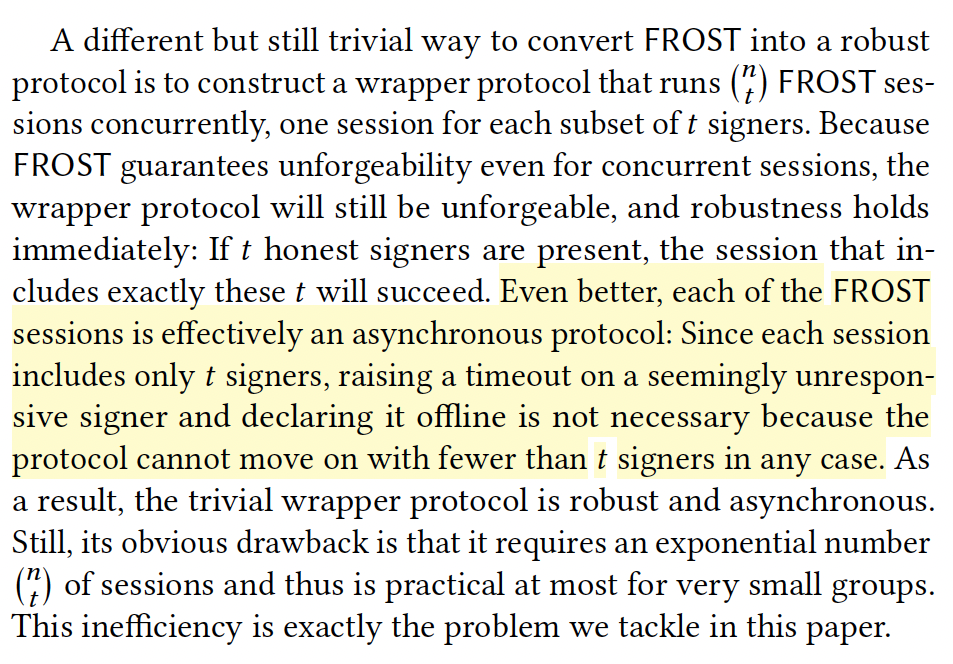
\includegraphics[width=1\linewidth]{images/ROAST_wrapper.png}
    \caption{The trivial wrapper for FROST to make it robust is asynchronous.}
\end{figure}

\newpage

\subsection{Original FROST Paper}

\begin{figure}
    \centering
    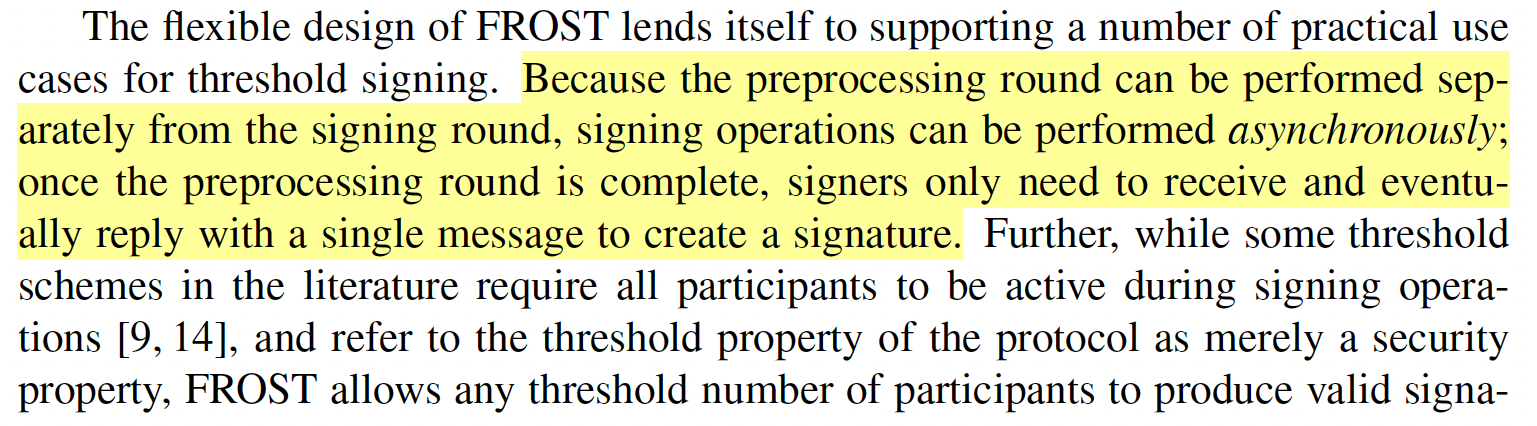
\includegraphics[width=1\linewidth]{images/FROST_async.png}
    \caption{This says only pre-processing FROST is asynchronous.}
\end{figure}

\begin{figure}
    \centering
    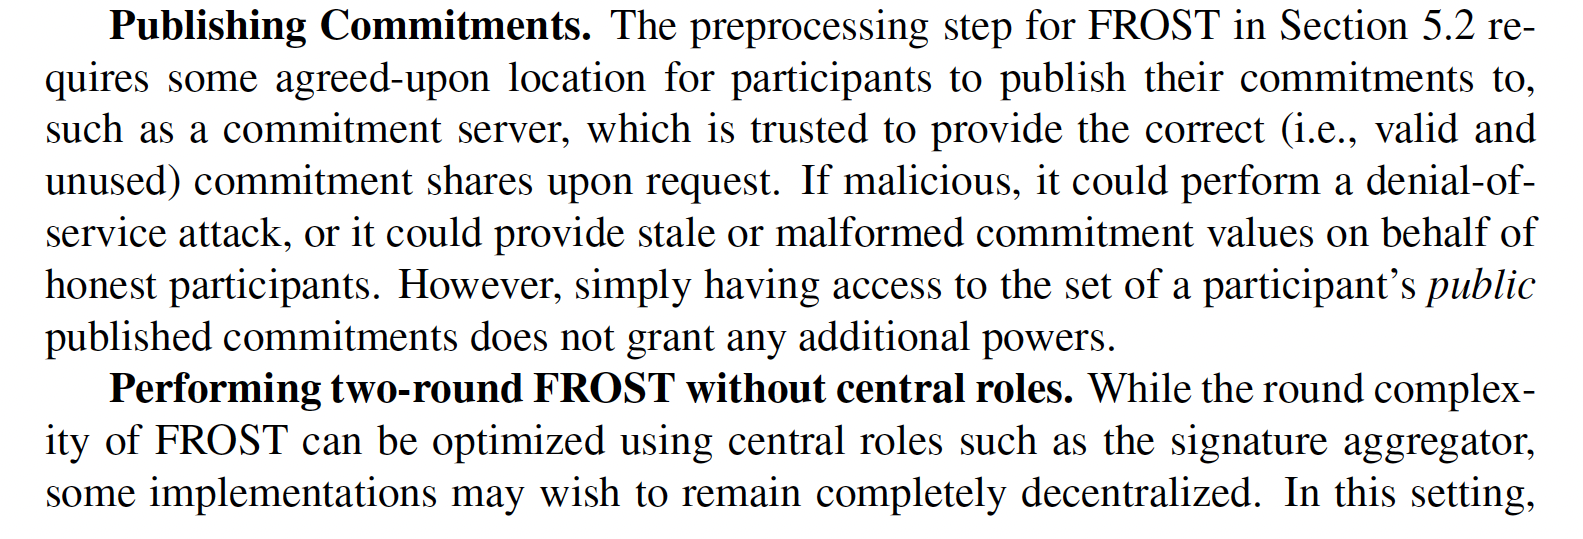
\includegraphics[width=1\linewidth]{images/FROST_aggregator.png}
    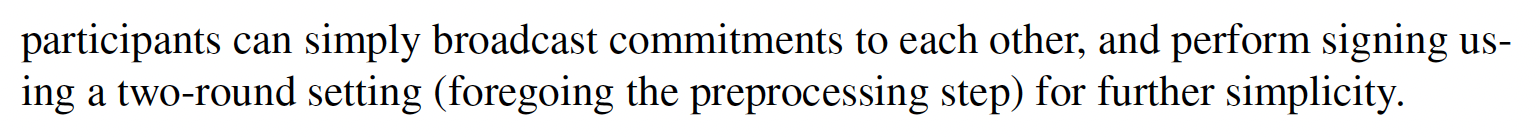
\includegraphics[width=1\linewidth]{images/FROST_aggregator2.png}
    \caption{FROST needs to be fully two rounds if broadcast is used instead of a signature aggregator.}
\end{figure}




